\subsection{Haptic sensitivity}
\label{Haptic sensitivity}

As the mechanoreceptors are enveloped in various skin layers, their sensitivity to vibrations will not be infinite. The strength of the sensation will depend on the frequency and amplitude of the vibration. The amplitude of the vibration can be considered in terms of the acceleration of the membrane-magnet system.
Previous works \cite{Vibrotactile_Sensitivity} found that, for a pulp contact area ranging from 53 to 176.7 mm\textsuperscript{2}, the threshold of detection of vibrations was between 0.1778 and 0.5623 m/s\textsuperscript{2} (in the work specified as 105-115 dB (re 1e-6m/s\textsuperscript{2})) for sinusoidal stimuli ranging from 100 to 250 Hz. \\+
For frequencies close to 125Hz the threshold should also lower as the finger pulp reaches its resonance frequency \cite{Skin_freqs_penetration}.

The study also highlights that the sensitivity depends on the constant pressure force applied on the skin in conjunction with the vibration.
They found that under active pressing force, the sensitivity threshold decreases to 0.027-0.143 m/s\textsuperscript{2} (in the work specified as 68.5-83.1 dB (re 1e-6m/s\textsuperscript{2})) for a constant applied force of 1.6N.

For higher pressure forces the sensitivity threshold decreases even further Fig.
\ref{fig:Vibrotactile_Sensitivity}.
\begin{figure}[H]
    \centering
    \resizebox{.8\linewidth}{!}{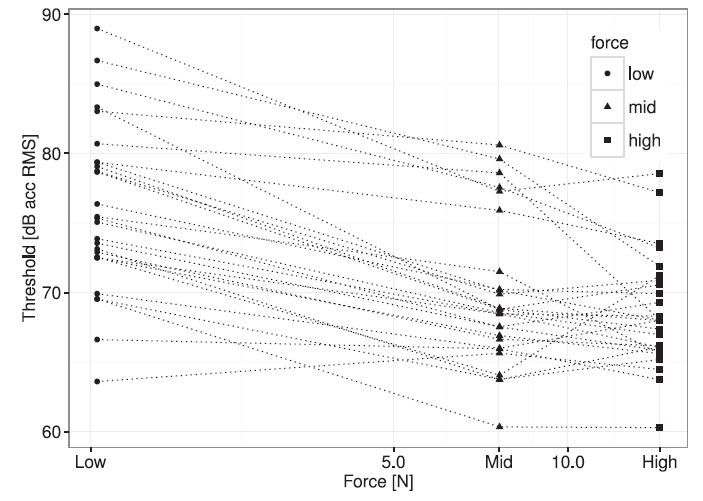
\includegraphics{Chapters/Chapter3/Haptics_Physics/Figures/vibr_thr_vs_pressure_force.png}}
    \caption{Vibrotactile Sensitivity as a function of the applied pressure force.}
    \label{fig:Vibrotactile_Sensitivity}
\end{figure}
